\chapter{Safety Plan Overview}

The safety of all team members is of the absolute highest priority for the Illinois Space Society Student Launch team. Should a situation arise in which a project-critical choice needs to be made, safety is considered before the success of the project. The safety officer this year is Zana Essmyer, who is overseeing a small team to conduct a thorough analysis of any hazards the team may encounter this year throughout the design, construction, assembly, and launches of the rocket and payload. Zana and the safety team are also implementing plans and procedures to minimize the risk of associated hazards.

This year, using a combination of in-person briefings, online classes and thorough documentation, the team is actively encouraging participation in the adherence to safety procedures. Safety training is required for any member that wishes to participate in construction sessions or attend a launch. By keeping lists of safety-trained members and having experienced members actively involved at every build session, the team can ensure that everyone working in lab spaces understands safety protocol for both day-to-day work and potential emergency situations. Forthcoming checklists will also be developed to ensure total safety during the off-pad, on-pad and post flight procedures.

\section{Emergency Preparedness}

Though the Illinois Space Society strives to maintain a safe working environment during all phases of the competition, the team also recognizes that accidents remain a possibility even with the strictest safety precautions in place. With this in mind, emergency preparedness forms another pillar of the team's safety plan. First aid kits are easily accessible in all of the team's main workspaces, and the safety officer has familiarized herself with their contents. The kits themselves are up-to-date and include wound dressings, antibiotic ointments, painkillers, and antihistamines. For any injuries requiring more than basic first aid, medical facilities are available both on and off the University of Illinois campus.

\section{Incident Reporting}

In the rare event that an accident requiring first aid occurs, the primary goal is always to care for and assist the injured team member. That said, once the incident has passed, the safety team's next priority is to actively prevent accident reoccurrence. Any incident is to be reported immediately to the safety officer, and from there it will be her responsibility to speak to those involved and determine the exact cause of the accident. Review of an incident will be considered complete once the safety officer has surveyed the scenario to her satisfaction and offered recommendations to the team leadership on how to prevent similar incidents in the future.

If an incident happens to occur, a series of actions will enact. The non-injured team member will assess the situation for any immediate dangers before contacting the Safety Officer, Technical Manager, and, if needed, emergency personnel. The Safety Officer will document the incident. The safety team will then take action to prevent further incidents.

\section{Equipment Training}

In order to provide team members with the experience necessary to operate a wide array of equipment and tooling, the safety team provides tutorial sessions on all machinery and tooling that may be used during the course of construction that is provided in the Nuclear Engineering Laboratory. To that end, the safety team has duplicated or adapted manufacturer-provided operating procedures for these tools and uploaded them to the team's shared drive for easy access. A collection of all training documents can be found in APPENDIX D: ISS Common Materials and Equipment Training with information included for the following devices:

\begin{itemize}[noitemsep]
    \item Full Spectrum Laser Professional Series CO2 48"$\times$36"  Cutter
    \item  Ultimaker 2 Extended 3D Printer
    \item Milwaukee Sawzall Reciprocating Saw
    \item DeWalt 18V Wireless Power Drill
    \item Dremel 8200-1/28 12-Volt Max Cordless Rotary Tool
    \item G5000 RocketPoxy
    \item Grizzly Model G7297 12" Disc Sander
    \item Water-Cooled Diamond Table Saw
    \item Grizzly H2936 Vacuum Sanding Table
    \item GMC 16" Scroll Saw
    \item JET 15" Bench Drill Press
    \item Soldering Station
    \item Miscellaneous Hand Tools (Screwdrivers, Hammer, Clamps, etc.)
\end{itemize}

In order to operate this machinery, a team member must attend tutorial sessions or receive training separately from a member of the safety team or team management. In providing and requiring these sessions, the team not only reduces the risk of mishaps due to misuse of equipment, but also ensures redundancy in knowledge of construction techniques. The Safety Officer will host tutorial sessions for ESPL machinery at the beginning of the semester for all members before access will be granted.

\section[NAR/TRA Procedures]{\gls{nar}/\gls{tra} Procedures}

The team will comply with the ``High Power Rocket Safety Code'' provided on the \gls{nar} website that has been effective since August 2012. The 13-step code and Minimum Distance Table on the website will be reviewed by the safety officer. All members on the team will be required to read the safety code online as it is a relatively short list of codes. The rules set forth by the \gls{nar} High Power Rocketry Code will always be respected and followed as they are set to ensure the safety of people and the environment. The safety officer, team manager, and sub-team managers will always make sure to comply with the safety code and ensure the rest of the team is properly complying. A copy of the \gls{nar} High Power Rocketry Code is included in this report as App.~\ref{App:Safety:NARCode}. Additionally, sections \todo[author=HE]{Add sec. on hazardous operations} and \todo[author=HE]{Add sec. on risk mitigation} elaborate on the hazardous operations and mitigation of risks. Hazardous materials and proper protocol is detailed under section\todo[author=HE]{Add sec. on hazardous materials}.

\paragraph{\gls{nar} Mentor.}

Mark Joseph will be the \gls{nar} mentor for the ISS Student Launch team for this year's competition. In addition to his longtime involvement in the high-power rocketry community, Mark has worked with the ISS team for several years now in the NASA Space Grant, Intercollegiate Rocket Engineering, and Student Launch Competitions.

\chapter{Risk Assessment Overview}

To better prepare for issues that inevitably arise during any project of large scale and to prioritize the team's time, the safety team has conducted a thorough risk analysis based on incident severity. The safety team analyzed risks to the project, the environment, and above all, the health of team members during the construction process. The team used \acrfullpl{rac} to evaluate the various hazards to both personnel and the project. Table~\ref{tab:level of risk and member requirements} introduces the risk matrix and the risk assessment codes that will be used to classify risks throughout the rest of the safety section. Risks are color-coded based on their severity, and  discusses the team's response to these various levels.  defines the levels of severity as it relates to personnel, project, and environmental health. Table 9 defines individual instance probability and probability of occurrence throughout the entire project timeline.

\begin{table}[H]
    \centering
    \caption{Level of risk and member requirements}
    \label{tab:level of risk and member requirements}
    \begin{tabularx}{0.8\linewidth}{X c c c c}
        \toprule
       \multirow{2}{*}{\textbf{Probability}} & \multicolumn{4}{c}{\textbf{Severity}} \\
       \cmidrule(l){2-5}
        & 1---Catastrophic & 2---Critical & 3---Marginal & 4---Negligible \\
       \midrule
       A---Frequent & \cellcolor{red!25} 1A & \cellcolor{red!25} 2A & \cellcolor{orange!25} 3A & \cellcolor{green!25} 4A \\
       B---Probable & \cellcolor{red!25} 1B & \cellcolor{red!25} 2B & \cellcolor{orange!25} 3B & \cellcolor{green!25} 4B \\
       C---Occasional & \cellcolor{red!25} 1C & \cellcolor{orange!25} 2C & \cellcolor{orange!25} 3C & 4C \\
       D---Remote & \cellcolor{orange!25} 1D & \cellcolor{orange!25} 2D & \cellcolor{green!25} 3D & 4D \\
       E---Improbable & \cellcolor{green!25} 1E & \cellcolor{green!25} 2E & \cellcolor{green!25} 3E & 4E \\
       \bottomrule
    \end{tabularx}
\end{table}

\chapter{Environmental Impact Analysis}

The Student Launch large rocketry project will consist of electronic parts, chemical elements, and many machined material components. The official rocket launch introduces two main risks, property damage and environmental contamination. In order to prevent property damage, the team will strictly adhere to NASA’s launch guidelines as well as the regulations detailed by the National Association of Rocketry. The team will also conduct rigorous testing before the official launch date to ensure the launch will not result in property damage. The team will ensure that all components of the rocket are retrievable and will land in the area designated by NASA.

Due to the composition of the rocket, the project introduces the risk of environmental contamination should the components prove to be irretrievable. Chiefly there is a risk of chemical contamination stemming from batteries on board and leftover rocket fuel. In order to mitigate this risk, the team will comply with all official regulations and testing standards. By ensuring the rocket is completely retrievable, the risk of environmental contamination is eliminated.

\chapter{STEM Engagement}

\section{Overview}

In order to maximize the positive impact that ISS has on local communities, the organization places an emphasis on educational outreach. With already planned outreach events, ISS expects to engage with over 21,000 students K-12, which meets the minimum of 200 individuals set by the official competition requirements. All outreach events will take place in the allotted window, after project acceptance and before the FRR due date.

\section{Past Outreach Opportunities}

\paragraph{Illinois Space Day.} Illinois Space Day (ISD) is the largest ISS event of the year, hosting K-8 students from local Illinois school districts for a day of enriching STEM activities. This year Illinois Space Day was held on October 5th from 8 am to 3 pm in the Digital Computer Laboratory at UIUC.

ISD included many fun and interactive engineering design activities for students to participate in like the Egg Drop Challenge and ISS Legos. Each year, ISD invites a keynote speaker to give a presentation about their work in the aerospace industry. ISD also included presentations from other aerospace student organizations and allowed attending K-8 students a chance to have a group discussion with ISS volunteers during a student panel. Members of the ISS Student Launch team have been involved in the planning of ISD 2020, with more members who volunteered to mentor and run the event. An impression of this year's ISD can be found in Fig.~\ref{fig:Safety:ISD}.

\begin{figure}[H]
	\centering
	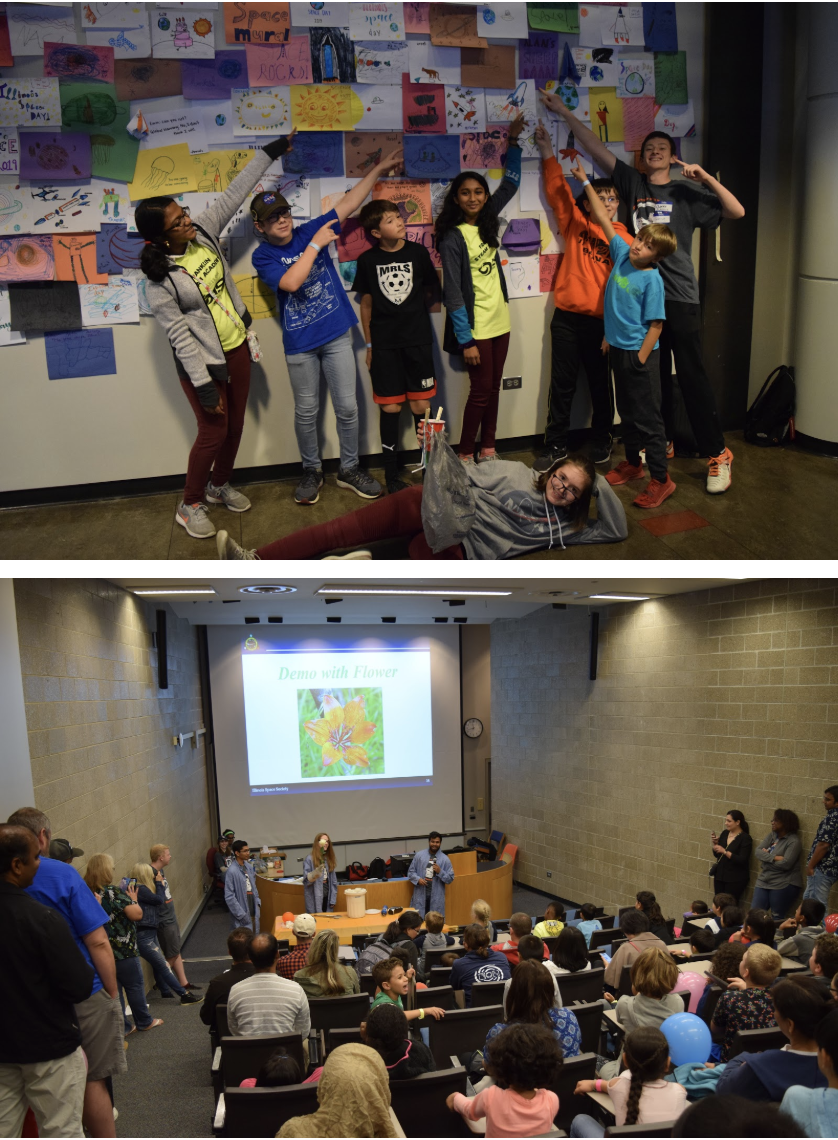
\includegraphics[width=0.4\linewidth]{img/Safety/isd}
	\caption{Top: Students and mentors show off the student-made space mural
Bottom: Students attend a liquid nitrogen demonstration}
	\label{fig:Safety:ISD}
\end{figure}

\section{Planned Outreach Opportunities}

\section{Engineering Open House.} Another major opportunity for engagement is the annual Grainger College of Engineering’s Open House on March 27th and 28th. Each year at the Engineering Open House, thousands of students K-12 and their families are invited to UIUC to learn more about student STEM projects. The Grainger College of Engineering relies on student led organizations like ISS to develop and present interactive learning exhibits to the estimated 20,000 annual attendees. ISS actively participates in Engineering Open House, with popular exhibits that include; an orbit simulator, rocket surgery, and liquid nitrogen demonstrations. ISS members are charged with running these stations and teaching young students about our tech projects and introduce them to the marvels of space exploration.

This event is unique in its massive scale and breadth of engineering disciplines represented, allowing students to interact with the engineering community at UIUC and ask questions. Engineering Open House is a great way for the ISS Student Launch team to help introduce students from the local community to the possibilities of a career in STEM.
